\documentclass[11pt, a4paper]{article}
\usepackage[T2A]{fontenc}
\usepackage[utf8]{inputenc}
\usepackage[bulgarian]{babel}

%% Sets page size and margins
\usepackage[a4paper,top=3cm,bottom=3cm,left=3cm,right=3cm,marginparwidth=1.75cm]{geometry}

%% Useful packages
\usepackage{amsmath, amssymb, amsthm,calc,mathabx}
\usepackage{systeme}
\usepackage{graphicx}
\usepackage[colorinlistoftodos]{todonotes}
\usepackage[colorlinks=true, allcolors=black]{hyperref}
\usepackage{wrapfig,lipsum,booktabs}
\usepackage{enumitem}
\usepackage{float}
\usepackage{fmtcount}
\usepackage{multicol}
\usepackage{breqn}
\usepackage{setspace}
\usepackage{hyperref}
\usepackage{mathtools}
\usepackage {tikz}
\usetikzlibrary {positioning}
\usetikzlibrary{shapes.geometric}
\graphicspath{
	{Graphics/}
	{Graphics/BackupFunction/}
}
\newtheorem{theorem}{Theorem}

\newtheorem{lemma}{Lemma}
\newtheorem{prop}{Property}
\newtheorem*{remark}{Remark}

\theoremstyle{definition}
\newtheorem{definition}{Дефиниция}

\setlength{\columnsep}{1cm}
\setlength{\parindent}{1em}

\newcommand\blfootnote[1]{%
	\begingroup
	\renewcommand\thefootnote{}\footnote{#1}%
	\addtocounter{footnote}{-1}%
	\endgroup
}

\begin{document}
\begin{titlepage}
	\newcommand{\HRule}{\rule{\linewidth}{0.5mm}}
	\centering
	\textsc{\LARGE Млади таланти 2020}\\[1cm]
	\HRule\\[1 cm]
	{\huge\bfseries Устойчиви стратегии за архивиране}\\[0.5 cm] 
	\HRule\\
	\vfill
	\Large
	\textit{Автор:}
	\textsc{Никола Стайков}\\
	\vspace{2cm}
	\Large
	\textit{Ръководител:}
	\textsc{Явор Папазов}\\
	
\includegraphics[width=0.5\textwidth]{Innofair_logo.png}\\
	\vfill	
	{\large\today}   
	\vfill
\end{titlepage}

\tableofcontents
\newpage
\begin{abstract}
		Архивите представляват резервни копия на данни, които да бъдат възстановени в случай на злополука. Те са основното средство за защита срещу рансъмуер и други видове вируси, както намаляват рисковете от критични щети в случай на природни бедствия. На свой ред обаче могат да представляват съществен разход за големите компании поради огромното количество данни, които трябва да бъдат подсигурени. Това на свой ред поражда нуждата те да бъдат внимателно планирани. Настоящият проект разразглежда модел за архивиране на данни, състоящ се от пълни и инкрементални архиви, изчислявайки очакваната цена за възстановяване на данните и цената на съхранение. Корелацията между изгубените и възстановените данни е разгледана като фактор за формиране на цената на възстановяване Процесът по възстановяване е пресъздаден и анализиран чрез визуализация на Python и Монте Карло симулация. Моделът намира оптимална стратегия за архивиране при предварително въведени параметри, характеризиращи работата на конкретния клиент. Оптималните стратегии при различни конфигурации са изведени и сравнени.
\end{abstract}

\section{Въведение}
		Настоящият проект изгражда теоретичен математически модел с цел намирането на оптимална стратегия за архивиране. Моделът включва два вида архиви, пълни и инкрементални. Параметрите, които оптимизираме, са интервалите в дни между видовете архиви. Структурата от архиви между два пълни архива образува цикъл, който се повтаря неопределено. Той се дефинира изцяло от два интервала - между пълните и между инкременталните архиви. Получените резултати се базират на два основни компонента- възможността за провал при възстановяваване на данните (различна за видовете архиви) и цената за съхранение на данните. Ефектите на двата компонента се изчисляват самостоятелно като след това се обединяват посредством константа, показваща отношението между цената на данните и техния размер. Подобни модели са правени и в миналото \cite{qian2010optimal}, \cite{nakamura2003optimal}, но те разглеждат само цената за съхранение, при неконстантна скорост на генериране на данни. Там интервалът между два последователни архива не е константен. Разгледана е и възможността за корелация между възстановените и загубените данни. За пълното разбиране на проекта са нужни базови знания по статистика и вероятности, използвани са стандартни означения и дефиниции.\newpage

\section{Теоретична постановка}
	Настоящият модел е създаден с цел да изчисли и оптимизира очакваната цена като сума на два компонента, цена на възстановяване и цена на съхранение. Двата за разгледани поотделно като очакваната цена за всеки от тях е изчислена при различни стратегии на архивиране. Моделът обединява двата компонента чрез безразмерна величина, отразяваща отношението между стойността на генерираните данни и цената за тяхното съхранение. Тъй като тя се променя в зависимост от компанията, моделът отчита спецификата на работа на ползвателя.
	\subsection{Възстановяване}
		Ще разглеждаме архивът като структура от данни със следните компоненти:
		$$
		b
		\begin{cases}
		d \text{: датата на създаването на архива като разлика в дни от първия архив}\\
		p \text{: вероятността възстановяването да е неуспешно}\\
		r \text{: цената за опит за възстановяване}
		\end{cases}
		$$
		Разгледани са два вида архиви:
		\begin{enumerate}
			\item Пълен архив: запазва копие на цялата база данни до момента на създаване
			\item Инкрементален архив: запазва само промените спрямо последния архив
		\end{enumerate}
		Архивите от конкретен вид имат обща вероятност за провал и цена за опит за възстановяване. \par
		За да може един инкрементален архив да е успешен, трябва всички инкрементални архиви преди него до успешен пълен архив също да са успешни, както и самият пълен архив.\par
		Важно е да се отбележи, че цената на данните в случая не съвпада с пазарната им такава. Това е така поради субективната им важност за компанията. Това е и причината в описания модел цената на данните да се разглежда като вечно увеличаваща се величина и за целите на изследването "скоростта на работа" на компанията се счита за константа. Ще я означим с $w$.\par
		Цената на процеса по възстановяване ще разглеждаме като сума от два фактора:
		\begin{enumerate}
			\item Цената на изработването на загубените данни, означена с $W$
			\item Цената на процеса по възстановяването, означена с $R$.
		\end{enumerate}
		Дефинираме $W = \Delta tw$, където с $\Delta t$ означаваме разликата в дни между датата на създаване на последния успешно възстановен архив и датата на възстановяване, и $R = \sum_{i=1}^{n} r_i$, където броят опити за възстановяване е $n$.
		Нека разликата в дни между първия направен архив и датата на възстановяване е $T$. В случай, че никой от пълните архиви не се окаже успешен, трябва да прераборим и данните преди първия направен архив. Нека той е направен $Т_0$ дни след началото на генериране на данни. Тогава в този случай $\Delta t= T+T_0$.\par
		\newpage
	\subsection{Съхранение}
		В даден момент всеки архив генерира цена за съхранение в зависимост от размера си и колко дълго е съхраняван. Приемаме, че размерът на генерираните данни, $S$, е пропорционален на стойността на генерираните данни $W$, описана в предишния параграф. Тогава $Sc=W$, където $c$ е константа. Цената за съхранение на количеството данни, които се генерират за един ден за един ден означаваме със $s$. Така приносът на всеки архив към цената на съхранение може да се опише чрез формулата:
		$$
			P_S = S\Delta ts,
		$$
		където с $\Delta t$ е означено времето, през което е бил съхраняван архивът.\par\noindent
		Пълните и инкременталните архиви имат различен принос, тъй като размерът на едните е фиксиран, докато на другите постоянно расте.
\section{Цена на възстановяване}\label{Recovery_price}
	В тази част е описана компонентата от модела, свързана с цената на процеса по възстановяването на данни и последващата преработка на загубените данни.
	\subsection{Пълни архиви}
				Когато разглеждаме само пълни архиви, моделът е разпределение на Бернули с краен брой опити, а именно броят пълни архиви. Спираме, когато успеем да намерим успешен архив, започвайки от последния и вървейки към първия. Да дефинираме свойствата на пълен архив($b_F$):
				$$
				b_F
				\begin{cases}
				p_F: \text{вероятността за провал}\\
				r_F: \text{цената за опит за възстановяване}\\
				t_F: \text{дните между два последователни пълни архива}\\
				\end{cases}
				$$
				Нека $k$ е броят пълни архиви направени преди деня на атаката. Тогава:
				$$
				k = \left \lfloor{\frac{T}{t_F}}\right \rfloor + 1
				$$
				Сега можем да дефинираме очакваната цена на възстановяване:
				\begin{equation}
					\label{eq:1}
					E(T) = p_F^{k}\left(W_T + kr_F\right) + \displaystyle \sum_{i=0}^{k-1} 	(1-p_F)p_F^{i}\left( \left (\left\{ \frac{T}{t_F}\right \} + i\right)t_Fw + (i+1)r_F \right )
				\end{equation}
				Направените изчисления са ключови поради невъзможността инкременталните архиви да бъдат възстановени без работещ пълен архив и следователно намирането на такъв е първият ни приоритет. Сега можем да разгледаме инкременталните архиви при работещ пълен архив.
\newpage
			\subsection{Инкрементални архиви с работещ пълен архив}
				Ще разгледаме случая, когато имаме работещ пълен архив и се опитваме да възстановив допълнителни данни чрез инкрементални архиви.\\
				Нека дефинираме свойствата на инкременталните архиви ($B_I$) по подобен начин:
				$$
				b_I
				\begin{cases}
					p_I: \text{вероятността за провал}\\
					r_I: \text{цената за опит за възстановяване}\\
					t_I: \text{дните между два последователни инкрементални архива}\\
				\end{cases}
				$$
				Нека с $T_F$ да означим разликата в дни между денят на атаката и датата на успешния пълен архив и с $l$ да означим броят инкрементални архиви, които трябва да разгледаме. Имаме две опции за $l$ в зависимост от това дали последният пълен архив е бил успешно възстановен:
				$$
				l=
				\begin{cases}
				\left\lfloor \frac{T_F}{t_I}\right \rfloor \text{, ако } T_F<t_F\\
				\left\lfloor \frac{t_F}{t_I}\right \rfloor -1 \text{, ако } T_F>t_F\footnotemark\\
				\end{cases}
				$$
				\footnotetext{Можем да опитваме да възстановим само инкрементални архиви, предхождащи следващият пълен архив}
				Да отбележим, че това последният пълен архив да е успешен е еквивалентно на $T_F<t_F$.\par
				Сега сме в точно обратната ситуация спрямо миналата част. Процесът по възстановяване на инкрементални архиви продължава докато не се натъкнем на провал, тъй като това би означавало, че всички следващи инкрементални архиви също са неизползваеми. С това намаляме $W$, тъй като в началната позиция сме готови да преработим данните до датата на успешния пълен архив. Сега сме готови да изчислим очакваната цена:
				\begin{equation}
					\label{eq:2}
					f(T_F) = (1-p_I)^l((T_F-t_Il)w + r_Il) + \displaystyle \sum_{i=0}^{l-1} (1-p_I)^{i}p_I((T_F-t_Ii)w + r_I(i+1))
				\end{equation}
				Сега знаем колко ще намалее цената на възстановяването, когато използваме инкрементални архиви, и можем да построим цялостния модел, използвайки уравнения \ref{eq:1} и \ref{eq:2}.
			\subsection{Очаквана цена на възстановяване}
				Към всяко събираемо в уравнение \ref{eq:1} трябва да добавим ефектът на инкременталните архиви и получаваме нови събираеми от вида:
				$$
				P(W + R),
				$$
				където $P$ е вероятността определена комбинация от събития да се случи, $W$ е цената на данните, които трябва да бъдат създадени наново, а $R$ е цената на процесът по възстановяването. Инкременталните архиви намаляват цената на данните, които трябва да бъдат създадени наново, но увеличават $R$. Както споменахме по-горе, има само един случай, вкойто броят инкрементални архиви, които трябва да имаме предвид е различен и той е именно този, в който последният пълен архив е възстановен успешно. Ако $i$-тият пълен архив е успешен\footnote{Това съответства на $i-1$-вото събираемо в сумата от формула \ref{eq:3}}:
				$$
				T_F=t_F\left(\left\{ \frac{T}{t_F} \right\} + i - 1\right)
				$$
				Комбинирайки уравнения \ref{eq:1} и \ref{eq:2} получаваме:
				\begin{equation}\label{eq:3}
				F(T) = p_F^{k}(W_T+kr_F) + \displaystyle\sum_{i=0}^{k-1}(1-p_F)p_F^{i}\left(f(T_F) + (i+1)r_F\right)
				\end{equation}
			\subsection{Корелация на данните}
				Тъй като между изгубените и оцелелите данни може да съществува връзка, въвеждаме функция, показващa отношението между скоростта на създаване на данни ($w$) и скоростта на тяхното възстановяване ($r$), зависеща от процента загубени данни, $x$\ref{Fig:Rec_rate}:
				$$
				\dfrac{r}{w} = g(x) = e^{1-x}
				$$
				Колкото повече данни сме изгубили, толкова по-близо е скоростта на възстановяване до скоростта на създаване. Ако моментът на възстановяване е $T$ и най-скорошният успешен архив е на дата $b_d$, то загубените данни са от $\Delta t = T - b_d$ дни, а $x = \dfrac{\Delta t}{T + T_0}$, където $T_0$ е броят дни преди първия архив.\\
				Ако последният успешно възстановен инкрементален архив е $i-$тият в цикъла си, то:
				$$x = \dfrac{T_F-t_Ii}{T + T_0}.$$
				Сега можем да заместим $w$ с $r=wg(x)$ в \ref{eq:2}, съответно и в \ref{eq:3}:
				\begin{equation}
				\label{eq:4}
				f(T_F) = (1-p_I)^l((T_F-t_Il)wg(x) + r_Il) + \displaystyle \sum_{i=0}^{l-1} (1-p_I)^{i}p_I((T_F-t_Ii)wg(x) + r_I(i+1)).
				\end{equation}
				
			\subsection{Симулация Монте Карло}
				Направена бе симулация от тип Монте Карло на Python, която генерира случайни процеси на възстановяване на данни с описаната структура на архивите. Конструирана е графика, \ref{Fig:MonteCarlo}, която показва цената на възстановяване за единичните процеси спрямо датата на възстановяване.
\newpage
	\section{Цена на съхранение}\label{Storage_price}
			Цената на съхранение се генерира от вече създадените архиви като за всеки индивидуално зависи от вида му и датата на създаване. Цената за съхранение на определено количество  данни за един ден ще означим със $s$. За целите на модела приемаме, че размерът на данните $S$ е пропорционален на цената за създаването им. За да отразим това взаимоотношение въвеждаме константата $c = \dfrac{W}{S}$.\par
			Нека в даден момент от създаването на първият архив $Т$ искаме да изчислим приносът на пълен архив, създаден $d$ дни след направата на първия архив. Броят дни на генериране на данни преди първия архив ще означим с $T_0$. Тогава архивът има размер $S=\dfrac{W}{c}=\dfrac{w\Delta t}{c} = \dfrac{w(T_0 + d)}{c}$, където $w$ e скоростта на работа от предишната компонента. Цената за съхранението му за ден е $s=\dfrac{w}{c}$ и сме го съхранявали $T-d$ дни, поради което конкретният пълен архив е генерирал цена за съхранение:
			$$
				\dfrac{w^2}{c^2}(T_0 + d)(T-d).
			$$
			Инкременталните архиви от друга страна имат фиксиран размер $\dfrac{w}{c}t_I$. Така приносът към цената за съхранение на инкременталните архиви се променя само от времето, през което са били съхранявани, а именно $T-d$. Окончателно приносът на инкрементален архив, направен $d$ дни след първия архив е: 
			$$
					\dfrac{w^2}{c^2}t_I(T-d).
			$$
			Ако с $B_I$ означим множеството на инкременталните архиви, а с $B_F$ множеството на пълните архиви, то цената за съхранение е:
			\begin{equation}\label{eq:5}
				\left(\displaystyle\sum_{b\in B_F}\dfrac{w^2}{c^2}(T_0 + d_b)(T-d_b)\right) + 	\left(\displaystyle\sum_{b\in B_I}\dfrac{w^2}{c^2}t_I(T-d_b)\right).
			\end{equation}
			За $b\in B_F$, $d_b$ приема стойности:
			$$lt_F|\ l\in \left[0,\left\lfloor\dfrac{T}{t_F}\right\rfloor t_F\right],$$
			а при $b\in  B_I$:
			$$d_b= mt_F + nt_I|\ m\in \left[0, \left\lfloor\dfrac{T}{t_F}\right\rfloor\right],n\in \left[1, \left\lfloor\dfrac{t_F}{t_I}\right\rfloor\right].$$
			Замествайки в \ref{eq:5} получаваме
			\begin{equation}
				\left(\displaystyle\sum_{l = 0}^{\left\lfloor\frac{T}{t_F}\right\rfloor t_F}\dfrac{w^2}{c^2}(T_0 + lt_F)(T-lt_F)\right) + \left(\displaystyle\sum_{m = 0}^{\left\lfloor\frac{T}{t_F}\right\rfloor}\displaystyle\sum_{n = 1}^{\left\lfloor\frac{t_F}{t_I}\right\rfloor}\dfrac{w^2}{c^2}t_I(T-mt_F + nt_I)\right)
			\end{equation}
			С това можем да намерим цената за съхранение на генерираните данни. Променяйки отношението между цената на съхранение и стойността на генерираните данни ($c$), можем да намерим оптимални стратегии за архивиране спрямо интервалите между последователни инкрементални и пълни архиви.
	\section{Резултати}
			Резултатите от модела са систематизирани в апендикса, сравнени са двата случая за вида данни, със и без корелация [\ref{table_clean}, \ref{table_corr}]. Изведени са съответните най-добри стратегии. Архивите се пазят за определено време, което зависи от вида на данните. Известно е обаче, че средния период на запазване е от 1 до 3 месеца \cite{Gloukhovtsev}, \cite{Schepers}. Затова и стратегиите се оценяват като се изчислява средният им резултат за стойностите на $T$ в този интервал. Тъй като моделът цели да раграничи различните стратегии, то можем да считаме $w$ за единица и да мерим резултата в дни работа. Тоест цената, изведена от модела, всъщност представлява цената на данните, които бихме изработили за съответния брой дни. Показано е и отношението на цените при най-добрите стратегии, съответно в двата случая, за различни стойности на $c$ \ref{Fig:Corr_vs_clean}. Важно е да се отбележи, че тези стратегии не са еднакви, но за едно и също $c$ винаги оптималната стратегия при корелация на данните се представя по-добре от оптималната стратегия без корелация на данните.\par 
			Беше построен модел за изчисляване на очакваната цена при възстановяване на данни и съхранението им със и без корелация на създаваните данни. Беше направена и анализирана симулация от тип Монте Карло, която демонстрира реалния процес на възстановяване.
	\section{Бъдещо развитие}
		Авторът разглежда няколко посоки за бъдещото развитие на пректа, а именно:
		\begin{itemize}
			\item неконстантна скорост на работа 
			\item корелация между оцелелите и изгубените данни
			\item нетривиални връзки между стойността на данните и размера им
		\end{itemize}
	\section{Благодарности}
		Искам да благодаря на своя ментор, Явор Папазов, и на Константин Делчев за безотказната помощ в избора на темата на проекта и последващото му развитие, за снабдяването ми с всички нужни материали за запознаването ми с темата, както и за изслушването на въпросите ми. Искам също да благодаря на Станислав Харизанов за професионалните съвети и за препоръките за развитие на проекта.
\newpage
\bibliographystyle{unsrt}
\bibliography{Bibliography}
\section{Апендикс}
	\subsection{Графики}
		По-долу е показана графика, символизираща начина, по-който обхождаме направените архиви, търсейки последния работещ.
		\begin{center}
		\begin{tikzpicture}
		[every node/.style={inner sep=0pt}]
		\node (1) [circle, minimum size=50.0pt, fill=teal, line width=0.625pt, draw=black] at (50.0pt, -130pt)  {};
		\node (2) [circle, minimum size=31.25pt, fill=lime, line width=0.625pt, draw=black] at (135pt, -130pt)  {};
		\node (3) [circle, minimum size=31.25pt, fill=lime, line width=0.625pt, draw=black] at (220pt, -130pt)  {};
		\node (4) [circle, minimum size=31.25pt, fill=lime, line width=0.625pt, draw=black] at (305pt, -130pt)  {};
		\node (5) [circle, minimum size=50.0pt, fill=teal, line width=0.625pt, draw=black] at (390pt, -130pt)  {};
		\draw [line width=0.625, ->, >=latex, color=black] (1) to  (2);
		\draw [line width=0.625, ->, >=latex, color=black] (2) to  (3);
		\draw [line width=0.625, ->, >=latex, color=black] (3) to  (4);
		\draw [line width=0.625, ->, >=latex, color=black] (4) to  (5);
		\end{tikzpicture}
		\end{center}
		Използвайки уравнения \ref{eq:1} и \ref{eq:3}, можем да построим графика на очакваната цена с и без използването на инкрементални архиви.
		\begin{figure}[H]
			\begin{minipage}{1.0\textwidth}
				\centering
				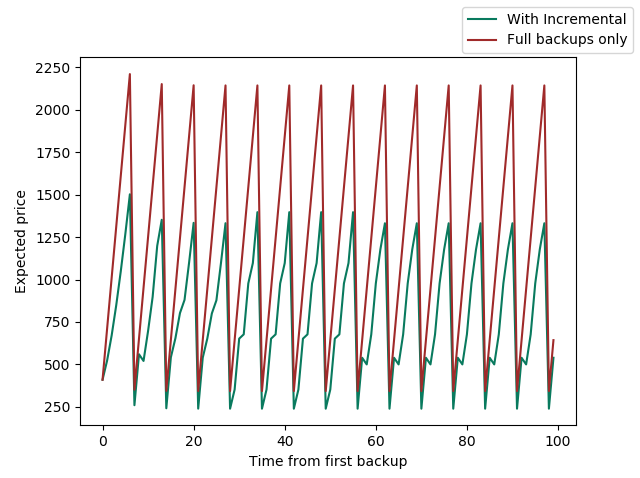
\includegraphics[width=0.7\textwidth]{Weekly_full.png}
				\caption{Само пълни архиви и целия модел}\label{Fig:FullWeekly}
			\end{minipage}
		\end{figure}
		На следващата графика е показано как се изменя отношението между цената на създаване и цената за възстановяване(повторно създаване) на данни в зависимост от количеството загубени:
		\begin{figure}[H]
			\begin{minipage}{1.0\textwidth}
				\centering
				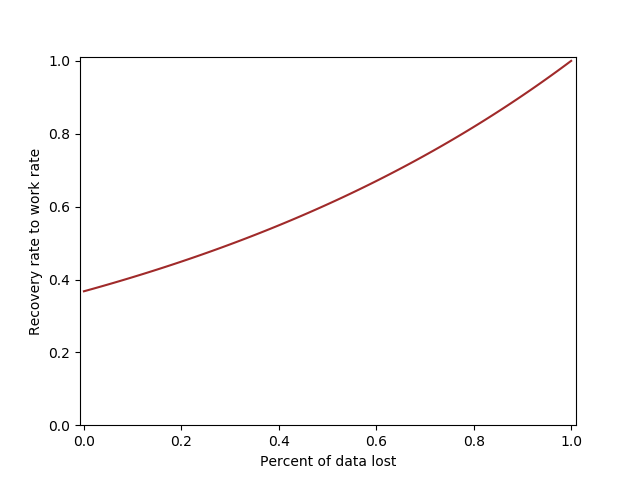
\includegraphics[width=0.7\textwidth]{Recovery_rate.png}
				\caption{Връзка между $w$ и $r$}\label{Fig:Rec_rate}
			\end{minipage}
		\end{figure}
		Графиката по-долу е генерирана от симулацията Monte Carlo и случайните процеси на възстановяване.
		\begin{figure}[H]
			\begin{minipage}{1.0\textwidth}
				\centering
				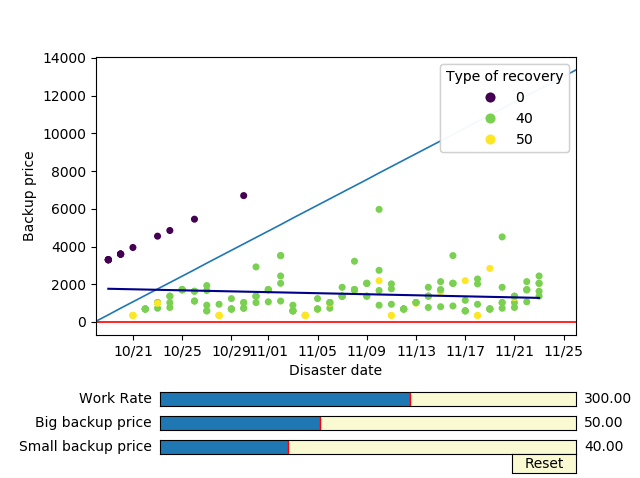
\includegraphics[width=0.7\textwidth]{Weekly_full_carlo.png}
				\caption{Симулация Монте Карло}\label{Fig:MonteCarlo}
			\end{minipage}
		\end{figure}
		\blfootnote{Във фигура \ref{Fig:FullWeekly} и фигура \ref{Fig:MonteCarlo} данните са за седмичен пълен архив и ежедневен инкрементален}
		Цветовете във фигура \ref{Fig:MonteCarlo} показват вида на последния успешно възстановен архив, пълен, инкрементален или несъществуващ. Беше генерирана линейна регресия на данните, която показва как ефектът от начално неподсигурените данни намалява с времето, тъй като цената при провал се изчилсява като цената за преработването на всички данни, които компанията е генерирала.\par
		По-долу е показана графика на резултатите на част от възмоните стратегии при $c = 1000$
		\begin{figure}[H]
			\begin{minipage}{1.0\textwidth}
				\centering
				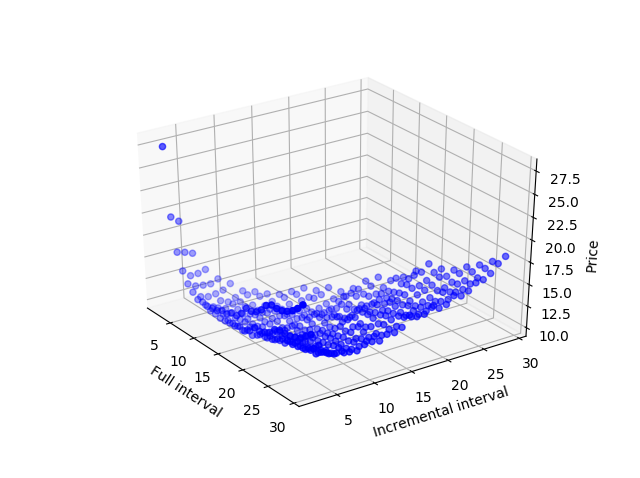
\includegraphics[width=0.7\textwidth]{3d_all_1.png}
				\caption{Визуализация за $c=1000$}\label{Fig:Whole_model}
			\end{minipage}
		\end{figure}
		Следващата графика показва отношението на цените на най-добрите стратегии с и без корелация на данните при различни стойности на $c$.
		\begin{figure}[H]
			\begin{minipage}{1.0\textwidth}
				\centering
				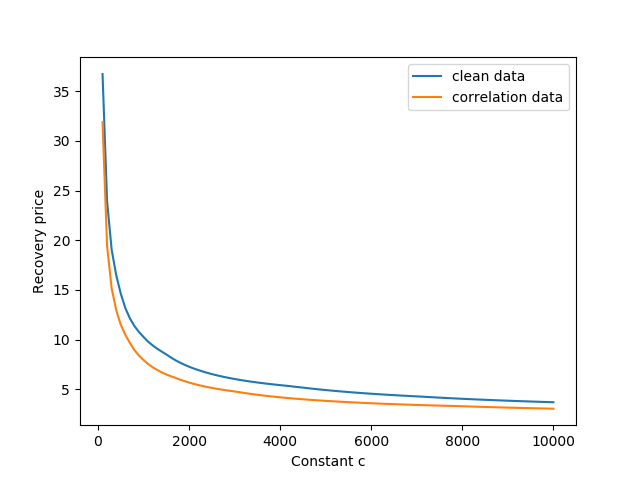
\includegraphics[width=0.7\textwidth]{correlation_vs_clean.png}
				\caption{Сравнените на цените в двата случая}\label{Fig:Corr_vs_clean}
			\end{minipage}
		\end{figure}
		Забелязваме, че при ниски $c$ разликата е съществена и постепенно намалява. Това се дължи на факта, че при по-големи $c$ оптималните стратегии включват по-чести архиви и съответно шансът да загубим голяма част от данните намалява.
\newpage	
	\subsection{Резултати}
			Таблиците по-долу обобщават получените резултати за най-добри стратегии при различни стойности на $c$ в двата разглеждани случая.\par
			При корелация на данните:
			\begin{center}\label{table_corr}
			\begin{tabular}{| l | l | l | l |}
				\hline
				Константа $c$ & Пълен интервал & Инкрементален интервал & Цена\\ \hline
				100 & 29 & 15 & 31.86\\ \hline
				200 & 29 & 16 & 19.40\\ \hline
				300 & 27 & 14 & 15.16\\ \hline
				400 & 27 & 14 & 12.97\\ \hline
				500 & 26 & 9 & 11.5\\ \hline
				600 & 21 & 12 & 10.49\\ \hline
				700 & 16 & 9 & 9.66\\ \hline
				900 & 16 & 9 & 8.39\\ \hline
				1000 & 16 & 6 & 7.94\\ \hline
				1600 & 16 & 6 & 6.31\\ \hline
				1700 & 11 & 6 & 6.15\\ \hline
				3000 & 11 & 6 & 4.78\\ \hline
				3100 & 8 & 5 & 4.71\\ \hline
				7899 & 8 & 5 & 3.31\\ \hline
				8000 & 6 & 3 & 3.29\\ \hline
				10000 & 6 & 3 & 3.05\\ \hline
			\end{tabular}
			\end{center}
		Без корелация на данните:
		\begin{center}\label{table_clean}
			\begin{tabular}{| l | l | l | l |}
				\hline
				Константа $c$ & Пълен интервал & Инкрементален интервал & Цена\\ \hline
				100 & 29 & 16 & 36.72\\ \hline
				200 & 29 & 10 & 23.9\\ \hline
				300 & 26 & 9 & 19.04\\ \hline
				400 & 21 & 8 & 16.49\\ \hline
				500 & 17 & 6 & 14.62\\ \hline
				600 & 16 & 6 & 13.18\\ \hline
				900 & 16 & 6 & 10.76\\ \hline
				1000 & 13 & 5 & 10.26\\ \hline
				1300 & 13 & 5 & 9.08\\ \hline
				1400 & 11 & 3 & 8.79\\ \hline
				1500 & 8 & 3 & 8.51\\ \hline
				4100 & 8 & 3 & 5.37\\ \hline
				4200 & 6 & 3 & 5.32\\ \hline
				4500 & 6 & 3 & 5.17\\ \hline
				4600 & 5 & 2 & 5.11\\ \hline
				6999 & 5 & 2 & 4.29\\ \hline
				7100 & 4 & 2 & 4.26\\ \hline
				10000 & 4 & 2 & 3.7\\ \hline
			\end{tabular}
		\end{center}
	
\end{document}